\documentclass[11pt,oneside,a4paper,final]{article}

\usepackage{fancyhdr}
\usepackage{lastpage}

\pagestyle{fancy}

\renewcommand{\headrulewidth}{0.0pt}

\lhead{}
\chead{}
\rhead{}
\lfoot{}
\cfoot{Page {\thepage} of \pageref{LastPage}}
\rfoot{}

\usepackage{longtable}

\usepackage[T1]{fontenc}  
\usepackage{textcomp}  
\usepackage{lmodern}  

\usepackage[style=numeric,backend=biber]{biblatex}
% \usepackage[style=numeric]{biblatex}
\bibliography{programmer_guide}
\usepackage[hidelinks=true]{hyperref}
\usepackage[paper=a4paper,margin=1.6cm]{geometry}	% 1 inch margins all around
\usepackage[british=nohyphenation]{hyphsubst}
\usepackage[british]{babel}
\usepackage{graphicx}
\usepackage[caption=false,font=normalsize,labelfont=sf,textfont=sf]{subfig}
\usepackage{color}

\definecolor{mygreen}{rgb}{0,0.6,0}
\definecolor{mygray}{rgb}{0.5,0.5,0.5}
\definecolor{mymauve}{rgb}{0.58,0,0.82}

\usepackage{listings}
 \lstset{ %
  literate={"}{\textquotedbl}1,
  backgroundcolor=\color{white},   % choose the background color; you must add \usepackage{color} or \usepackage{xcolor}
  basicstyle=\footnotesize,        % the size of the fonts that are used for the code
  breakatwhitespace=false,         % sets if automatic breaks should only happen at whitespace
  breaklines=true,                 % sets automatic line breaking
  captionpos=b,                    % sets the caption-position to bottom
  commentstyle=\color{mygreen},    % comment style
%   deletekeywords={...},            % if you want to delete keywords from the given language
%   escapeinside={\%*}{*)},          % if you want to add LaTeX within your code
  extendedchars=true,              % lets you use non-ASCII characters; for 8-bits encodings only, does not work with UTF-8
  frame=single,                    % adds a frame around the code
  keepspaces=true,                 % keeps spaces in text, useful for keeping indentation of code (possibly needs columns=flexible)
  keywordstyle=\color{blue},       % keyword style
  language=C++,                 % the language of the code
%   morekeywords={*,...},            % if you want to add more keywords to the set
  numbers=left,                    % where to put the line-numbers; possible values are (none, left, right)
  numbersep=5pt,                   % how far the line-numbers are from the code
  numberstyle=\tiny\color{mygray}, % the style that is used for the line-numbers
  rulecolor=\color{black},         % if not set, the frame-color may be changed on line-breaks within not-black text (e.g. comments (green here))
  showspaces=false,                % show spaces everywhere adding particular underscores; it overrides 'showstringspaces'
  showstringspaces=false,          % underline spaces within strings only
  showtabs=false,                  % show tabs within strings adding particular underscores
  stepnumber=1,                    % the step between two line-numbers. If it's 1, each line will be numbered
  stringstyle=\color{mymauve},     % string literal style
  tabsize=2,                       % sets default tabsize to 2 spaces
  title=\lstname                   % show the filename of files included with \lstinputlisting; also try caption instead of title
}

\usepackage[acronym,toc]{glossaries}
\makeglossaries
% \phantomsection
% \addcontentsline{toc}{section}{Acronyms}
% \section*{Acronyms}
% \begin{footnotesize}
% \begin{acronym}[TDMA]

% \newacronym{2D}{2D}{two-dimensional}
\newacronym{3D}{3D}{three-dimensional}
\newacronym{FBO}{FBO}{frame buffer object}
\newacronym{FLTK}{FLTK}{Fast Light Toolkit}
\newacronym{GLEW}{GLEW}{OpenGL Extension Wrangler Library}
\newacronym{GLSL}{GLSL}{OpenGL Shading Language}
\newacronym{GLU}{GLU}{OpenGL Utility Library}
\newacronym{GLUT}{GLUT}{OpenGL Utility Toolkit}
\newacronym{GPU}{GPU}{Graphics Processor Unit}
% \newacronym{GUI}{GUI}{graphical user interface}
% \newacronym{Gzip}{Gzip}{GNU zip}
% \newacronym{ITK}{ITK}{Insight Segmentation and Registration Toolkit}
\newacronym{keV}{keV}{kiloelectron volt}
% \newacronym{MXE}{MXE}{M cross environment}
\newacronym{STL}{STL}{STereoLithography}
\newacronym{SVN}{SVN}{Subversion}
\newacronym{VBO}{VBO}{vertex buffer object}
% \newacronym{VTK}{VTK}{Visualization Toolkit}
% 


\title{gVirtualXRay -- Tutorial 01}
\author{Dr Franck P. Vidal}
\date{19\textsuperscript{th} March 2014}

\begin{document}
 \sloppy

\maketitle

\newpage
\phantomsection
\addcontentsline{toc}{section}{Table of contents}
\tableofcontents

\newpage
\phantomsection
\addcontentsline{toc}{section}{List of figures}
\listoffigures

% \newpage
% \phantomsection
% \addcontentsline{toc}{section}{List of tables}
% \listoftables

\newpage
\phantomsection
\addcontentsline{toc}{section}{List of listings}
\lstlistoflistings

\newpage

\section{Introduction}

The complete source code of this tutorial is available in \verb+example/src/tutorial_01.cxx+. 
It shows how to build a basic simulation pipeline and display the simulation setup using OpenGL. 
Basic knowledge of OpenGL and \Gls{GLUT} is a pre-requisite. 
The gVirtualXRay library is built using modern programming paradigm. 
Errors are handles using C++ exceptions. 
In the OpenGL code, the fix rendering pipeline and direct rendering have both been avoided. 
Depreciated functions and features have also been avoided. 
In this tutorial, some of these functionalities are still in used to lighten the tutorial. 
For example, the matrix stacks are used and the fix rendering pipeline is used too.

It is an introductory tutorial, for more details, the reader may refer to the code (it is well documented) and the Doxygen documentation. 

The tutorial is organised as follows:
Section~\ref{sec:Header inclusion} shows the header files to include. 
Section~\ref{sec:Name Spaces} shows some of the name spaces that can be included to lighten the code. 
How to set up all the main components of the simulation is describe in Section~\ref{sec:Setting Components of the X-Ray Simulation}.


\section{Header inclusion}
\label{sec:Header inclusion}

\lstinputlisting[firstline=32, lastline=58, caption=Header inclusion., label=lst:header]{../../../examples/src/tutorial_01.cxx}

Listing~\ref{lst:header} shows i) the macros that have to be defines to include OpenGL core profile hears and ii) the header files that need to be included to build a simple program based on the GLFW library~\cite{GLFW}. 
\begin{itemize}
% \item \verb+glew.h+ is the main header file from the \Gls{GLEW} . 
% It is required to include this file. 
% \Gls{GLEW} is used to handles \glspl{VBO}, \glspl{FBO}, and the \gls{GLSL}. 
% It has to be included before any other OpenGL header inclusion\ e.g.~\Gls{GLUT}.
% \item \verb+glut.h+ is the main \Gls{GLUT} header file.
 \item \verb+GL3_PROTOTYPES+ is a macro that ensures that we are using opengl's core profile only. It has to be included before any other OpenGL header inclusion.
 \item \verb+GL_GLEXT_PROTOTYPES+ is a macro that ensures that we are using opengl's core profile only. It has to be included before any other OpenGL header inclusion.
 \item \verb+GLFW_INCLUDE_GLCOREARB+ is a macro that tells GLFW to include the OpenGL core profile header. It has to be included before any other OpenGL header inclusion.
 \item \verb+glfw3.h+ is the main GLFW header file.
 \item \verb+iostream+ is used for output streams.
 \item \verb+exception+ is used for C++ exceptions.
 \item \verb+Types.h+ defines new types, e.g.~\verb+RATIONAL_NUMBER+, \verb+VEC2+, \verb+VEC3+ and \verb+MATRIX4+ to name a few.
 \item \verb+Units.h+ defines units such as metre, kilometre, electronvolt, kiloelectron volt, gram, kilogram, etc.
 \item \verb+PolygonMesh.h+ corresponds to a class used to handle \Acrshort{3D} triangle meshes.
 \item \verb+XRayBeam.h+ corresponds to a class used to manage X-Ray beams. The beam spectrum is discretised into energy channels.
 \item \verb+XRayDetector.h+ corresponds to a class that handles virtual X-Ray detectors.
 \item \verb+XRayRenderer.h+ is used to compute X-Ray images on the \Gls{GPU}.
 \item \verb+Shader.h+ corresponds to a class that handles \Gls{GLSL} programs.
 \item \verb+buildCube.h+ is used to create the triangle mesh of a cube.
\end{itemize}


\section{Name Spaces}
\label{sec:Name Spaces}

\lstinputlisting[firstline=64, lastline=65, caption=Name spaces., label=lst:name space]{../../../examples/src/tutorial_01.cxx}

Listing~\ref{lst:name space} shows the name spaces that can be selected. 
\begin{itemize}
 \item \verb+gVirtualXRay+ is used to defined all the components of the X-ray simulation. 
 	It also includes graphics elements such as \verb+PolygonMesh+ and utilities such as \verb+Exception+. 
 \item \verb+std+ is used for output streams and exceptions.
\end{itemize}


\section{Setting Components of the X-Ray Simulation}
\label{sec:Setting Components of the X-Ray Simulation}

Figure~\ref{fig:scene} illustrates the main components of the simulation. 
\begin{figure}[tbh]
 \centering
 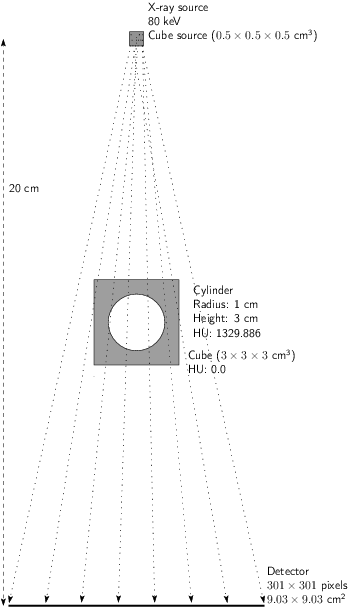
\includegraphics[width=0.5\textwidth]{scene.eps}
 \caption{\label{fig:scene} Definition of the main components needed to simulated X-ray images.}
\end{figure}

\lstinputlisting[firstline=77, lastline=83, caption=Declaration of the simulation components., label=lst:Global variables]{../../../examples/src/tutorial_01.cxx}

Four of them have to be defined to simulate X-Ray images:
\begin{enumerate}
 \item The detector (its position, orientation, number of pixels and the size of pixels); and
 \item The source (it includes the shape and position of the source);
 \item The beam (its energy spectrum);
 \item The scanned objects (their topologies, positions, orientations and material properties).
\end{enumerate}

To facilitate their integration into the GLFW example, they are declared as global variables (see Listing~\ref{lst:Global variables}).
\verb+g_sample_rotation_matrix+ is the modelling matrix that is used to transform the scanned object. 
By default it is a identity matrix. 
It could be used to move, rotate and scale the object. 
The \verb+Matrix4x4+ class provides such functionalities. 


\subsection{X-Ray Detector}

\lstinputlisting[firstline=407, lastline=426, caption=Setting up the X-ray detector., label=lst:Detector]{../../../examples/src/tutorial_01.cxx}

Listing~\ref{lst:Detector} shows how to initialise the detector. 
Four attributes have to be set:
\begin{enumerate}
 \item Number of pixels of the detector;
 \item Size of pixels (in unit of length);
 \item Position of the detector;
 \item Orientation of the detector.
\end{enumerate}

\textbf{Note: see how lengths are set in order to internally store them all in the same unit, e.g.} \verb+320.0 * mm+\textbf{, or} \verb+10.0 * cm+\textbf{.}

\subsection{X-Ray Source}

\lstinputlisting[firstline=429, lastline=436, caption=Setting up the X-ray source., label=lst:Source]{../../../examples/src/tutorial_01.cxx}

Listing~\ref{lst:Source} shows how to set the position and shape of the source. 
In this case, the shape corresponds to an infinitely small point. 
Other shapes can be chosen. % (see Section~\ref{sec:Source Shapes})


\subsection{Beam Spectrum}

\lstinputlisting[firstline=439, lastline=446, caption=Setting up the spectrum of the incident beam., label=lst:Beam spectrum]{../../../examples/src/tutorial_01.cxx}

Listing~\ref{lst:Beam spectrum} shows how to set the position and shape of the source. 
In this case, the beam spectrum is monochromatic and the energy of all the photons is 80~\acrlongpl{keV} (~\acrshort{keV}). 
Polychromatism can be chosen, in which case a beam spectrum has to be loaded. % (see Section~\ref{sec:Beam spectrum}).

\textbf{Note: see how energies are set, e.g.} \verb+80.0 * keV+\textbf{ for 80~\acrshort{keV}.}

\subsection{Scanned Object}

%\lstinputlisting[firstline=80, lastline=81, caption=Global variables used to store the topology of the scanned objects., label=lst:Scanned object topology]{../../../examples/src/tutorial_01.cxx}

\lstinputlisting[firstline=449, lastline=475, caption=Setting up the properties of the scanned object., label=lst:Scanned object]{../../../examples/src/tutorial_01.cxx}

In most simulation cases, the topology of the scan objects will be stored in the main memory as an array of triplets of floating point numbers. 
Each triplet corresponds to a vertex. 
An index of vertices can also be given to reduce the memory consumption, and eventually speed-up the computations. 
This is a well known practice in computer graphics.
Two objects are considered here (see Listing~\ref{lst:Global variables}). 
The first one makes use of two arrays (one for vertices and one for indices); the second one makes use of a single array (for vertices).

Listing~\ref{lst:Scanned object} shows how to set the properties of the scanned objects. 
\verb+buildCube(...)+ is used to initialise the topology of the two scanned objects as cubes. 
The topology of each cube is then passed on to instances of \verb+PolygonMesh+. 
Note that in this case, the memory is managed by the calling program, not by the class instance. 
It is also possible to load \Gls{STL} binary files, in which case the \verb+PolygonMesh+ class instance will manage the memory. 

The next step is to set the material property (here the Hounsfield value). 


\subsection{Simulation Environment}

\lstinputlisting[firstline=478, lastline=491, caption=Setting up the simulation environment., label=lst:Simulation Environment]{../../../examples/src/tutorial_01.cxx}

Listing~\ref{lst:Simulation Environment} shows how to set the simulation environment. 
Only the OpenGL simulation has been implemented. 
For fast computation, use \verb+GL_RGB16F_ARB+; for accurate results, use \verb+GL_RGB32F_ARB+. 
This parameter controls the number of bits used by floating point number. 
Finally, the detector, source and geometries have to be registered. 
One may note that the biggest cube, which totally enclose the smaller one is used as \verb+OuterSurface+ (it would be the case of the skin surface in the case of a medical simulation).
The smaller one is used as \verb+InnerSurface+ (it would be the case of bones and internal organs in the case of a medical simulation).

\newpage
\section{Running the Simulation}

\lstinputlisting[firstline=383, lastline=390, caption=Running the simulation., label=lst:Running the simulation]{../../../examples/src/tutorial_01.cxx}

To run the simulation, call \verb+XRayRenderer::computeImage(...)+ with the scanned object transformation matrix as parameter (see Listing~\ref{lst:Running the simulation}). 
It may be useful to call \verb+XRayRenderer::normalise()+ to make sure that the X-ray image is normalise before it is displayed. 
The image can be displayed in negative mode, or not. 
To enable and disable this mode, use \verb+XRayRenderer::useNegativeFilteringFlag(boolean_flag)+.

\lstinputlisting[firstline=240, lastline=289, caption=Display callback., label=lst:Display callback]{../../../examples/src/tutorial_01.cxx}
Listing~\ref{lst:Display callback} shows the \Gls{GLUT} display callback. 
One may note that the X-ray beam is displayed using transparency. 
It is the reason why it is displayed last. 
Figure~\ref{fig:tutorial 01 screenshot} shows the corresponding rendering.
\begin{figure}[tbh]
 \centering
 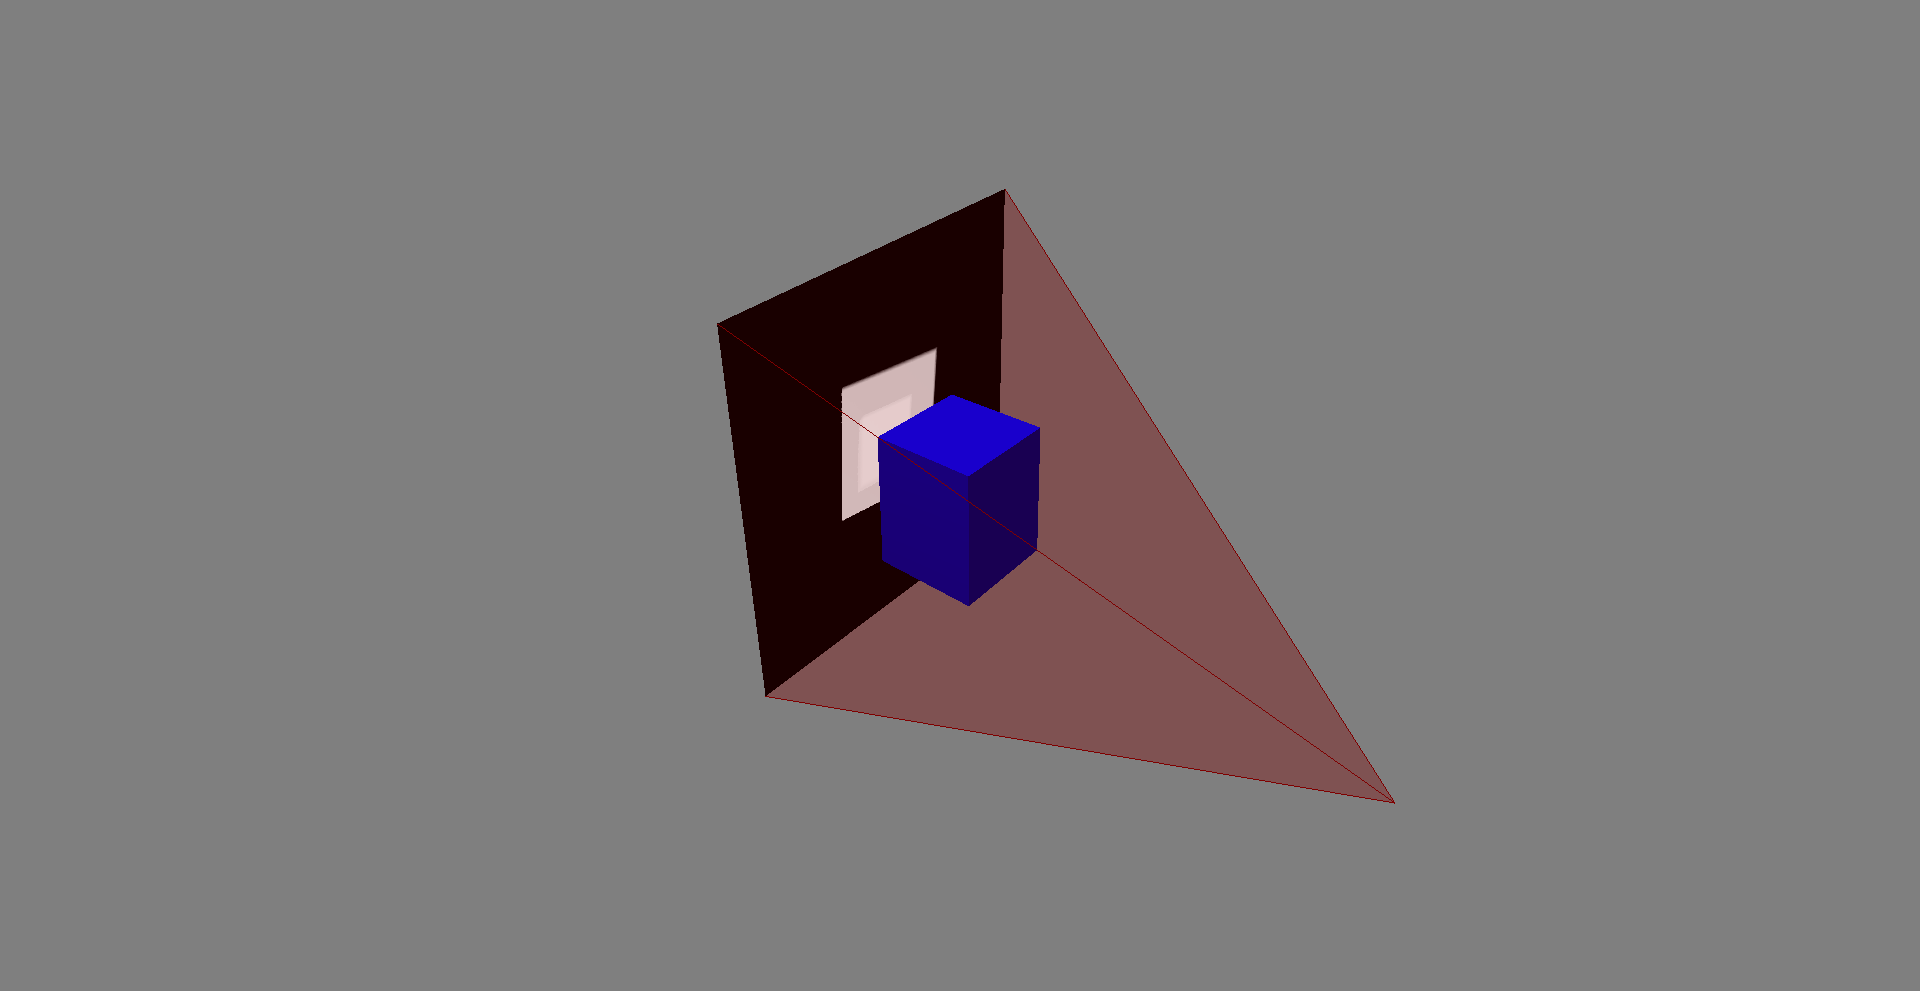
\includegraphics[width=0.5\textwidth]{tutorial_01.png}
 \caption{\label{fig:tutorial 01 screenshot} OpenGL rendering.}
\end{figure}

\section{Next Tutorial}

In the next tutorial:
\begin{itemize}
 \item  You will see how to get rid of OpenGL's fixed pipeline (which is now depreciated). 
 
 \item You will see how to get rid of OpenGL's matrix stack (which is now depreciated).

 \item We will see how to create an efficient mouse control to turn the \Acrshort{3D} scene, object, and detector (the detector does not have to be centered and orthogonal to the beam). 

 \item You will also see how to update the topology of the triangle meshes. 
 This is important in medical simulations with soft tissue deformations. 
\end{itemize}

\newpage
\printglossary[type=\acronymtype] 

% \newpage
% \phantomsection
% \addcontentsline{toc}{section}{References}
% \printbibliography


\end{document}
